\section{Diagrama de clases}

El diagrama de clases UML sirve para mostrar una vista estática de las clases de un sistema, sus atributos, métodos y relaciones entre objetos. Sirve para proporcionar una información general sobre la aplicación \cite{clase}.

Como se muestra en la figura \ref{fig:clases}, el simulador está compuesto por siete clases. De estas, únicamente la clase CASimulator se encuentra implementada en C++, por lo que se especifican su encapsulamiento y el tipo de sus variables.

El resto de las clases están desarrolladas en Python y se definen siguiendo la filosofía “pythónica”, en la cual “lo simple es mejor” \cite{pythonTutorial}.

\begin{figure}[H]
	\centering
	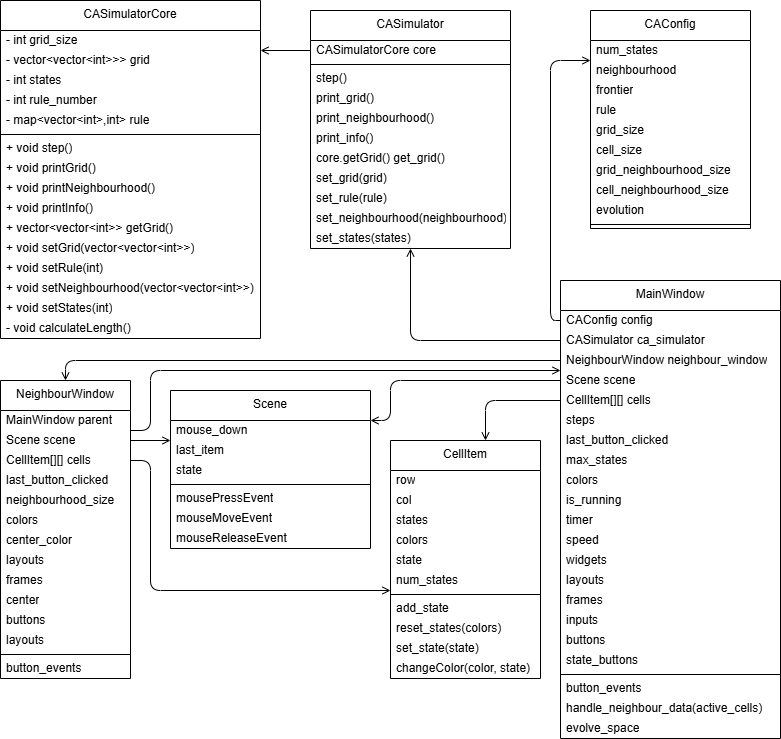
\includegraphics[width=0.9\linewidth]{img/uml_cd.png}
	\caption{Diagrama de clases.}
	\label{fig:clases}
\end{figure}